\documentclass[a4paper,12pt]{article}
\usepackage[utf8]{inputenc}

%  Русский язык
\usepackage{multirow}
\usepackage{wrapfig}
\usepackage[T2A]{fontenc}			% кодировка
\usepackage[utf8]{inputenc}			% кодировка исходного текста
\usepackage[english,russian]{babel}	% локализация и переносы

\usepackage{indentfirst} %Красная строка
\usepackage[a4paper,top=1.3cm,bottom=2cm,left=1.5cm,right=1.5cm,marginparwidth=0.5cm]{geometry}
\usepackage[usenames]{color}
\usepackage{colortbl}
\usepackage{csvsimple}
\usepackage{siunitx}

\addto\captionsrussian{\def\refname{5   Список используемой литературы}}

% Заметки
\usepackage{todonotes}

% Математика
\usepackage{amsmath,amsfonts,amssymb,amsthm,mathtools} 
\usepackage{hyperref}

\renewcommand{\AA}{\ensuremath{\mathring{A}}}

\begin{document}
\def\figurename{Рисунок}
\begin{titlepage}
\begin{center}
    {\large МОСКОВСКИЙ ФИЗИКО-ТЕХНИЧЕСКИЙ ИНСТИТУТ (НАЦИОНАЛЬНЫЙ ИССЛЕДОВАТЕЛЬСКИЙ УНИВЕРСИТЕТ)}
\end{center}
\begin{center}
    {\largeФизтех-школа биологической и медицинской физики}
\end{center}

\vspace{1cm}
{\huge
\begin{center}
    {\bf Лабораторная работа по оптике}\\
    \vspace{0.5cm}
    4.3.3. Исследование разрешающей способности микроскопа методом Аббе
\end{center}
}

\vspace{4cm}
\begin{flushright}
{\LARGE Выполнила студентка группы Б06-103:\\ Фитэль Алена \\}

\end{flushright}
\vspace{9cm}
\begin{center}
    Долгопрудный, 2023 г.
\end{center}
\end{titlepage}
\newpage


\section{Аннотация}

\textbf{Цель работы}: определение дифракционного предела разрешения объектива микроскопа.

\textbf{В работе используются}: лазер; кассета с набором сеток разного периода; щель с микрометрическим винтом; оптический стол с набором рейтеров и крепёжных винтов; экран; линейка.


\section{Теоретические сведения}
Для иммерсионного микроскопа разрешающая способность объектива при некогерентном освещении
\begin{equation}
\ell_{min} \approx \dfrac{0.61\lambda}{\sin u},
\end{equation}
где $u$ -- апертурный угол объектива микроскопа (угол между оптической осью и лучом, направленным из центра объекта в край линзы).

Метод Аббе для оценки разрешающей способности состоит в разделении хода лучей на две части: сначала рассматривается картина в задней фокальной плоскости $F$ объектива -- она называется первичным изображением. Это первичное изображение рассматривается как источник волн, создающий вторичное изображение в плоскости $P_2$, сопряжённой плоскости предмета.\\
Первичное изображение есть картина дифракции Фраунгофера (на дифракционной решётке), если её период $d$, то для направления максимальной интенсивности $\varphi_m$.

\begin{equation}
d \sin \varphi_m = m\lambda.
\end{equation}

При этом проходят пучки только с $\varphi_m < u$. Можно условием разрешения считать, что $u > \varphi_1$, иначе говоря:
$$
\sin u \geq \lambda/d.
$$
или
\begin{equation}
\label{equ:allow}
d \geq \dfrac{\lambda}{\sin u} \approx \dfrac{\lambda}{D/2f},
\end{equation}
где $D$ -- диаметр линзы, $f$ -- фокусное расстояние.\\
Сетку можно рассматривать как две перпендикулярные друг другу решетки, для максимумов которых выполняется соотношение
\begin{equation}
\begin{array}{c c}
d\sin \varphi_x = m_x \lambda, & d\sin \varphi_y = m_y \lambda. \\
\end{array}
\end{equation}


\begin{figure}[h!]
    \centering
    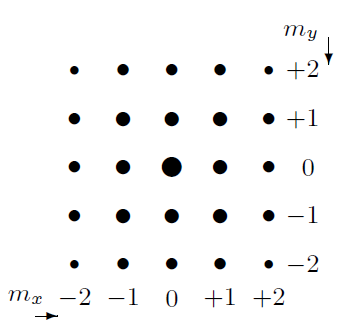
\includegraphics[width = 0.3\textwidth]{3.png}
    \caption{Дифракция Фраунгофера на двумерной решётке (сетке). Максимумы изображены кружками, размеры которых характеризуют интенсивности.}
    \label{fig:no_int}
\end{figure}\\


\newpage
\section{Экспериментальная установка}
\begin{figure}[h!]
	\centering
	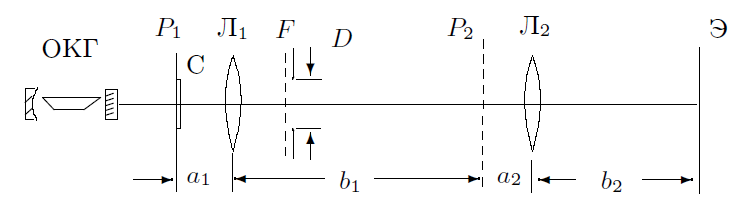
\includegraphics[scale=0.8]{4.png}
	\caption{Схема установки}
	\label{fig:stand}
\end{figure}
Схема установки приведена на Рис. \ref{fig:stand}. Предметом $P_1$ служат сетки в кассете $C$. Линза $\text{Л}_1$ длиннофокусная, а $\text{Л}_2$ короткофокусная. В $F$ устанавливаются диафрагмы $D$, с помощью сеток с разными $d$ и щелевой диафрагмы можно проверить соотношение (\ref{equ:allow}). Период сеток может быть измерен либо по расстоянию между дифракционными максимумами на экране, либо по увеличенному с помощью микроскопа изображению. Пространственную фильтрацию (получение наклонного изображение решётки) можно получить с помощью подбора угла наклона и ширины вспомогательной щели.

\section{Обработка результатов}

Запишем данные лабораторной установки:
\begin{table}[h!]
		\centering
		\begin{tabular}{|l|l|l|}
			\hline
			$\lambda$, нм & $f_1$, мм & $f_2$, мм \\ \hline
			532           & 110       & 25        \\ \hline
		\end{tabular}
	\end{table}
\subsection{Определение периода решеток по их пространственному спектру}

 Расстояние от дифракционной решетки до экрана $H = 1257 \pm 3$ мм. Для каждой сетки определим расстояние между вертикальными и горизонтальными максимумами $l_{v}$ и $l_{h}$соответственно , их количество ($n_{v}$  $n_{h}$) и посчитаем период вертикальных и горизонтальных сеток  $d_{v}$ и $d_{h}$ соответственно по формуле (2) с учётом $\varphi = \frac{l}{H}$ период решеток $d = \frac{n \lambda}{l}H$.. Результаты приведены в Таблице 1.
	
\begin{table}[h!]
\centering
\begin{tabular}{|r|r|r|l|r|r|r|r|r|}
\hline
\rowcolor[HTML]{FFFFFF} 
\multicolumn{1}{|l|}{\cellcolor[HTML]{FFFFFF}{\color[HTML]{032563} $N$}} & \multicolumn{1}{l|}{\cellcolor[HTML]{FFFFFF}{\color[HTML]{0E1116} $l_{h}$, мм}} & \multicolumn{1}{l|}{\cellcolor[HTML]{FFFFFF}{\color[HTML]{032563} $n_{h}$}} & {\color[HTML]{0E1116} $d_{h}$, мкм} & \multicolumn{1}{l|}{\cellcolor[HTML]{FFFFFF}{\color[HTML]{0E1116} $\delta d_{h}$, мкм}} & \multicolumn{1}{l|}{\cellcolor[HTML]{FFFFFF}$l_{v}$, мм} & \multicolumn{1}{l|}{\cellcolor[HTML]{FFFFFF}{\color[HTML]{032563} $n_{v}$}} & \multicolumn{1}{l|}{\cellcolor[HTML]{FFFFFF}$d_{v}$, мкм} & \multicolumn{1}{l|}{\cellcolor[HTML]{FFFFFF}{\color[HTML]{0E1116} $\delta d_{v}$, мкм}} \\ \hline
1                                                                        & 43                                                                              & 3                                                                           & 49.9                               & 1.2                                                                                    & 214                                                      & 4                                                                           & 13,38                                                    & \cellcolor[HTML]{FFFFFF}0.07                                                           \\ \hline
2                                                                        & 89                                                                              & 9                                                                           & 72.4                               & 0.8                                                                                    & 230                                                      & 9                                                                           & 30.00                                                       & \cellcolor[HTML]{FFFFFF}0.12                                                           \\ \hline
3                                                                        & 88                                                                              & 7                                                                           & 56.9                               & 0.6                                                                                    & 144                                                      & 11                                                                          & 54,7                                                     & \cellcolor[HTML]{FFFFFF}0.4                                                            \\ \hline
4                                                                        & 45                                                                              & 3                                                                           & 47.7                               & 1.1                                                                                    & 214                                                      & 4                                                                           & 13,38                                                    & \cellcolor[HTML]{FFFFFF}0.06                                                           \\ \hline
5                                                                        & 73                                                                              & 7                                                                           & 68.6                               & 0.9                                                                                    & 200                                                      & 8                                                                           & 28,62                                                    & \cellcolor[HTML]{FFFFFF}0.14                                                           \\ \hline
6                                                                        & 87                                                                              & 7                                                                           & 57.6                               & 0.7                                                                                    & 86                                                       & 7                                                                           & 58,2                                                     & \cellcolor[HTML]{FFFFFF}0.7                                                            \\ \hline
\end{tabular}
\caption{Период решеток, определенный методом пространственного спектра.}
\label{tab:my-table}
\end{table}

\subsection{Определение периода решеток по изображению, увеличенному с помощью микроскопа}
	
Запишем параметры настроенного микроскопа:
	\begin{table}[h!]
		\centering
		\begin{tabular}{|l|l|l|}
			\hline
			$a_1$, мм  & $b_1+a_2$, мм & $b_2$, мм  \\ \hline
			$130\pm 5$ & $1195\pm 5$    & $250\pm 5$ \\ \hline
		\end{tabular}
	\end{table}
\\Приняв $a_2 = f_2 = 25 \text{ мм}$ найдем: $b_1 = 380 \pm5$ мм. Увеличение получившейся системы:
	\[
		\Gamma = \frac{b_1b_2}{a_1a_2} = 92 \pm 4
	\]
	Запишем количество периодов сетки и расстояние между ними, а так же посчитаем период по формуле $d = l/(n\Gamma)$. Результаты измерений и расчетов приведены в Таблице 2.
	\begin{table}[h!]
\centering
\begin{tabular}{|r|r|r|r|r|}
\hline
\rowcolor[HTML]{FFFFFF} 
\multicolumn{1}{|l|}{\cellcolor[HTML]{FFFFFF}{\color[HTML]{032563} $N$}} & \multicolumn{1}{l|}{\cellcolor[HTML]{FFFFFF}{\color[HTML]{0E1116} $l_{v}$, мм}} & \multicolumn{1}{l|}{\cellcolor[HTML]{FFFFFF}{\color[HTML]{032563} $n_{v}$}} & \multicolumn{1}{l|}{\cellcolor[HTML]{FFFFFF}{\color[HTML]{0E1116} $d_{v}$, мкм}} & \multicolumn{1}{l|}{\cellcolor[HTML]{FFFFFF}{\color[HTML]{0E1116} $\delta d_{h}$, мкм}} \\ \hline
1                                                                        & 10                                                                              & 10                                                                          & 10.9                                                                            & 1.2                                                                                    \\ \hline
2                                                                        & 10                                                                              & 5                                                                           & 22                                                                              & 2                                                                                      \\ \hline
3                                                                        & 10                                                                              & 2                                                                           & 54                                                                              & 6                                                                                      \\ \hline
4                                                                        & 10                                                                              & 3                                                                           & 36                                                                              & 4                                                                                      \\ \hline
5                                                                        & 10                                                                              & 5                                                                           & 22                                                                              & 2                                                                                      \\ \hline
6                                                                        & 10                                                                              & 13                                                                          & 8.4                                                                             & 0.9                                                                                    \\ \hline
\end{tabular}
\caption{Период вертикальной решетки, определенный микроскопом.}
\label{tab:my-table}
\end{table}
		
	
\subsection{Определение периодов решеток по оценке разрешающей способности микроскопа}
	
	Если поместить в фокальную плоскость линзы Л$_1$ щелевую диафрагму, то при минимальном раскрытии, при котором будет видна решетка, ее период будет определяться:$d = \frac{2\lambda f_1}{D}$. Запишем результаты проведеных измерений и расчетов в Таблицу 3.

\begin{table}[h!]
\centering
\begin{tabular}{|r|r|r|r|r|r|r|}
\hline
\multicolumn{1}{|l|}{\cellcolor[HTML]{FFFFFF}{\color[HTML]{032563} $N$}} & \multicolumn{1}{l|}{$D$, мм} & \multicolumn{1}{l|}{$d$, мкм} & \multicolumn{1}{l|}{$1/D$, 1/мм} & \multicolumn{1}{l|}{\cellcolor[HTML]{FFFFFF}{\color[HTML]{0E1116} $\delta D$, мм}} & \multicolumn{1}{l|}{\cellcolor[HTML]{FFFFFF}{\color[HTML]{1F1F1F} $\delta d$, мкм}} & \multicolumn{1}{l|}{$\delta (1/D)$, 1/мм} \\ \hline
1                                                                        & \multicolumn{1}{l|}{-}       & \multicolumn{1}{c|}{-}        & \multicolumn{1}{c|}{-}           & -                                                                               & \multicolumn{1}{c|}{-}                                                              & \multicolumn{1}{c|}{-}                  \\ \hline
2                                                                        & 2,34                         & 50,0                          & 0,43                             & 0,01                                                                               & 0,2                                                                                 & 0,002                                    \\ \hline
3                                                                        & 1,35                         & 86,7                          & 0,74                             & 0,01                                                                               & 0,6                                                                                 & 0,005                                    \\ \hline
4                                                                        & \multicolumn{1}{l|}{-}       & \multicolumn{1}{c|}{-}        & \multicolumn{1}{c|}{-}           & -                                                                               & \multicolumn{1}{c|}{-}                                                              & \multicolumn{1}{c|}{-}                  \\ \hline
5                                                                        & 2,46                         & 47,6                          & 0,41                             & 0,01                                                                               & 0,2                                                                                 & 0,002                                    \\ \hline
6                                                                        & 1,78                         & 65,8                          & 0,56                             & 0,01                                                                               & 0,4                                                                                 & 0,003                                    \\ \hline
\end{tabular}
\caption{Периоды решеток по измерению размера диафрагмы.}
\label{tab:my-table}
\end{table}
	
Проверим справедливость этой формулы построив график $d = f(1/D)$. Угловой коэффициент прямой из МНК $k = (117 \pm 3) \cdot 10^{-9} \text{ м}^2$, в пределах погрешности он совпадает с теоретическим $2\lambda F_1 = 117 \cdot 10^{-9} \text{ м}^2$. Таким образом, теория Аббе подтвердилась.
\begin{figure}[h!]
		\centering
		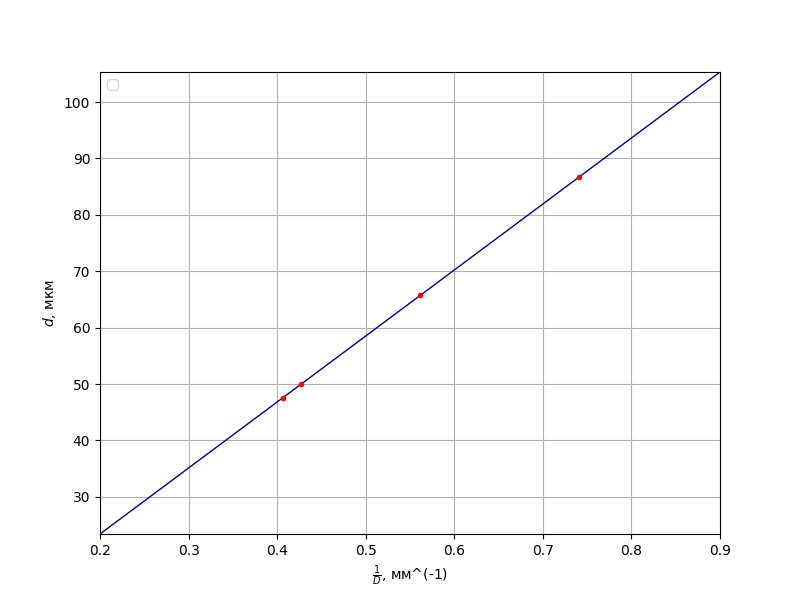
\includegraphics[scale = 0.6]{Figure_1.png}
	\end{figure}
\newpage

\subsection{Пространственная фильтрация и мультиплицирование}
\begin{enumerate}
\item  Для наблюдения пространственной фильтрации откроем щель так, чтобы она пропускала только максимум нулевого порядка и, поворачивая щель, наблюдаем за изменением картины. Полученные фото представлены на Рис 3.

\begin{figure}[h!]
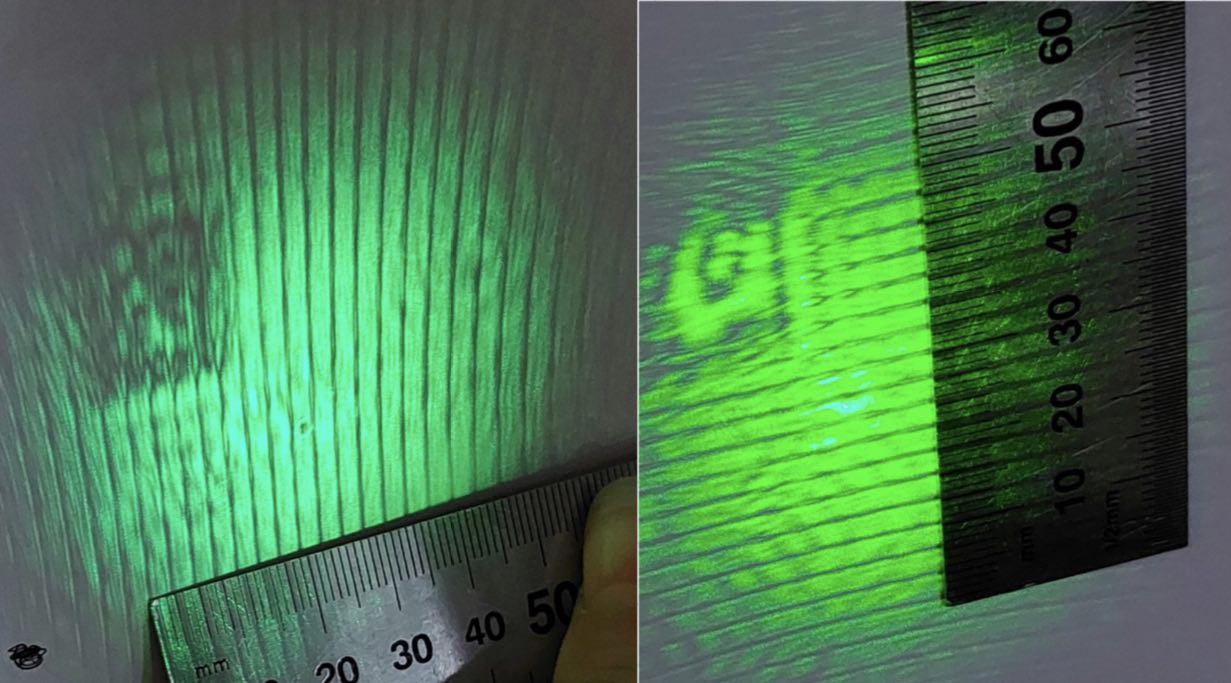
\includegraphics[scale=0.3]{14.jpg}
\centering
\caption{Слева направо: вертикальная щель $(m_x,0)$, горизонатальная щель $(0,m_y)$.}
\end{figure}
\item Поворачивая щель относительно оси, добьёмся того, чтобы щель занимала наклонное положение под $45^\circ$. Тогда будет осуществляться пространственная фильтрация, то есть выделение из спектра максимумов $m_x = m_y$ (диагональных максимумов).Полученные полосы располагаются под углом $45^\circ$. 
\item Пронаблюдаем мультиплицирование, то есть рассечение фурье-образа щели сеткой. Такой эффект создаётся, если в нашей установке поменять местами сетку и щель. Результат представлен на Рисунке 4.


\begin{figure}[h!]
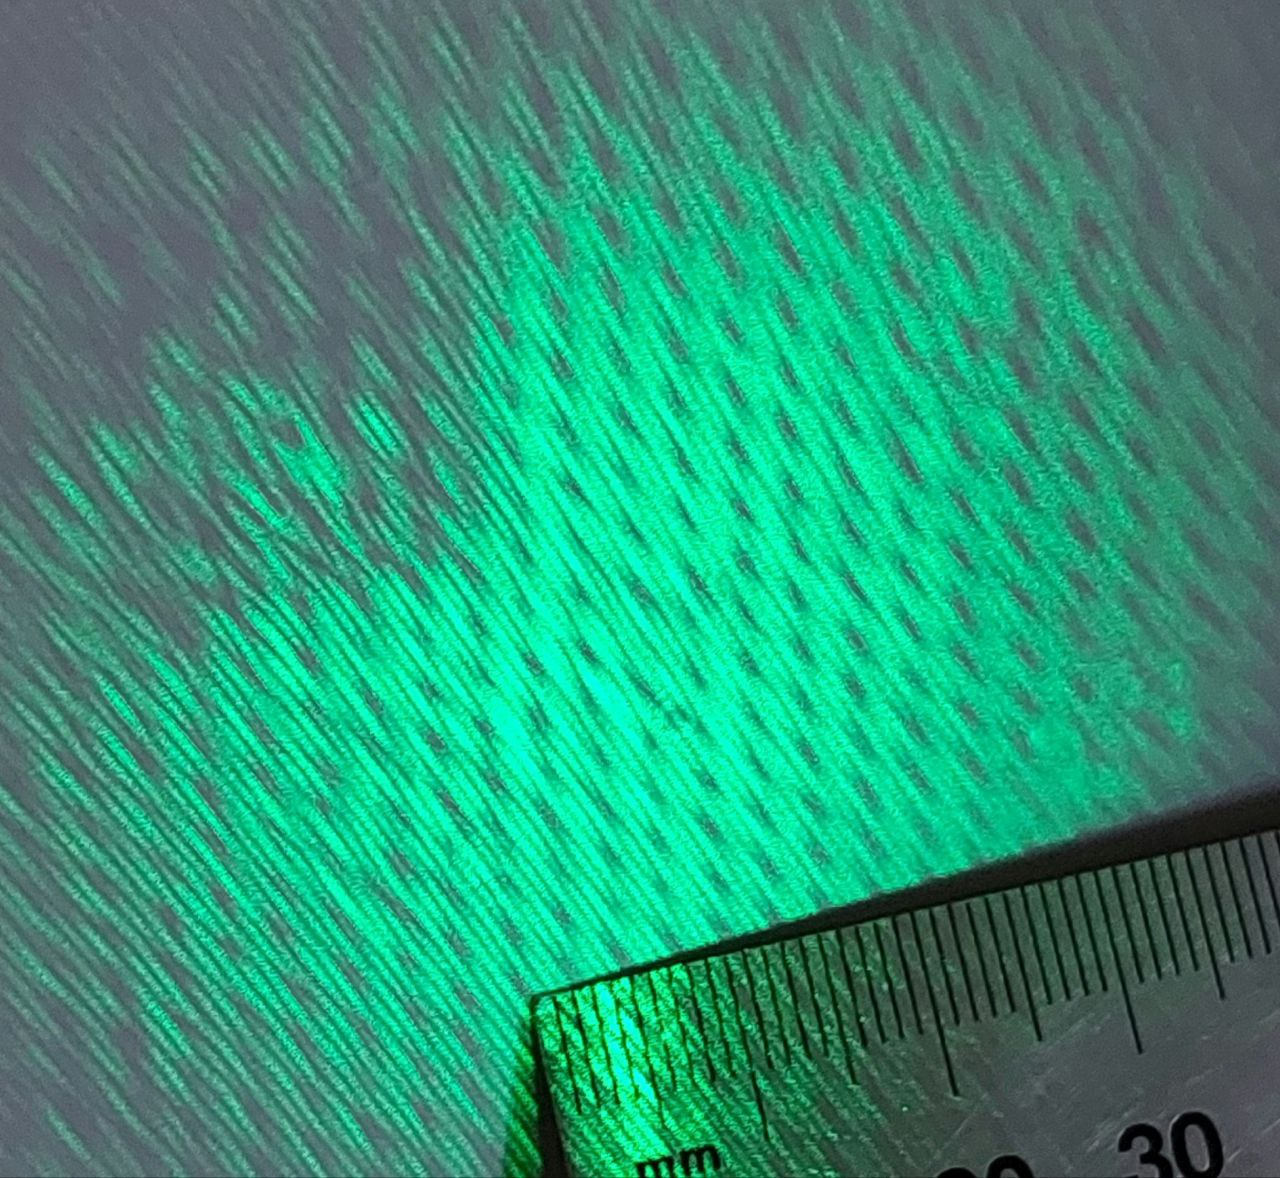
\includegraphics[scale=0.17]{13.jpg}
\centering
\caption{Явление мультипликации.}
\end{figure}

\end{enumerate}

\section{Вывод}


В ходе данной лабораторной работы были определены периоды дифракционных решёток различными способами. Полученные результаты отличаются друг от друга существенно, хотя имеют одинаковый порядок величины.Способ измерения с помощью дифракционной картины более точен, чем метод с моделью микроскопа, что связано с большой погрешностью расчёта расстояний между линзами и изображениями. Расхождение результатов в разных способах может быть связано с приближенным характером используемой теории, неточностью определения величин $a_2$ и $b_1$.
Построив график $d = f(1/D)$ мы убедились в справедливости формулы(), то есть проверка теории Аббе оказалась положительной. Качественно были  рассмотрены явления фильтрации и мультиплицирования.



\end{document}